\section{Desarrollo}
	Para la elaboración del programa, se realizó el siguiente diagrama que modela los estados y las transiciones que tiene la máquina.

	\begin{figure}[H]
		\begin{center}
			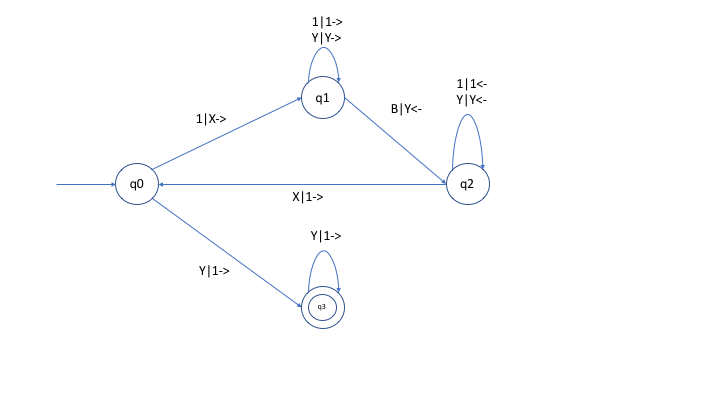
\includegraphics[scale=.4]{img/maquina.png}
			\caption{Estados y transiciones usados}
			\label{fig:maquina}
		\end{center}
	\end{figure}

	Posteriormente, para el modelado de la máquina de Turing se realizó la siguiente implementación en Python 3.7, la cual es una clase que sirve para trabajar con la misma:

	maquina.py
	\lstinputlisting[language=Python]{../maquina.py}

	Por si sola está máquina no tiene funcionalidad, por lo cual fue necesario el uso de la misma en otro archivo, el cual se encarga de manejar todo el funcionamiento del programa, como recibir la entrada (cadena de unos), y utilizar tkinter para realizar la animación de la máquina de Turing.
	\lstinputlisting[language=Python]{../main.py}